Parity games can be solved \textit{globally} or \textit{locally}; globally solving a parity game means that for every vertex in the game it is determined who the winner is. Locally solving a parity game means that for a specific vertex in the game it is determined who the winner is. For some applications of parity games, including model checking, there is a specific vertex that needs to be solved to solve the model checking problem so locally solving the parity game is sufficient for solving the original problem.

Similarly VPGs can be solved globally or locally where locally solving a VPG means determining for which configurations a certain vertex is won by player $0$ and for which configurations the vertex is won by player $1$.

Most parity game algorithms are concerned with global solving, when talking about solving a (V)PG we talk about globally solving it unless stated otherwise. For VPGs we consider a global and a local variant for every collective algorithm we are going to consider. When solving a VPG globally we might encounter significant differences in parts of the game or intermediate results between configurations that we don't encounter when solving it locally because we can terminate earlier. Therefore we hypothesize that the increase in performance between globally-collectively solving VPGs and locally-collectively solving VPGs is greater than the increase performance between globally-independently solving VPGs and locally-independently solving VPGs.

The two parity game algorithms introduced in the preliminaries (Zielonka's recursive algorithm and the fixed-point iteration algorithm) can be turned into local variants to solve VPGs locally and independently.

\subsection{Zielonka's recursive algorithm local}
\label{sec:zlnk_org_local}
To make Zielonka's recursive algorithm a local algorithm, we use the property that vertices won by player $\overline{\alpha}$ in game $G \backslash A$ are also won by player $\overline{\alpha}$ in game $G$. We use this property to, in some cases, not go into the second recursion because we already found the vertex. We extend the algorithm with two parameters, $v_0$ and $\Delta$. Vertex $v_0$ represents the vertex that we try to solve. Parameter $\Delta \subseteq \{0,1\}$ contains a set of players for which we try to find vertex $v_0$, if we find $v_0$ to be won by a player that is in $\Delta$ we are done for that recursion. However if we find vertex $v_0$ to be won by a player that is not in $\Delta$ we need to solve the entire game. The algorithm can make use of this to tell a recursive call it needs to find the vertex to be won by player $\overline{\alpha}$ in the subgame because then this vertex is also won by player $\overline{\alpha}$ in the game itself. If the vertex is not won by $\overline{\alpha}$ the entire game needs to be solved because the winning sets are required in the second recursion. Pseudo code for the algorithm is provided in algorithm \ref{alg_zlnk_local}.
\begin{algorithm}
	\caption{$\textsc{RecursivePGLocal}(\textit{PG } G = (V,V_0,V_1, E, \Omega),v_0,\Delta)$}
	\label{alg_zlnk_local}
	\begin{algorithmic}[1]
		\State $m \gets \min\{ \Omega(v)\ |\ v \in V\}$
		\State $h \gets\max\{ \Omega(v)\ |\ v \in V\}$
		\If{$h = m$ or $V = \emptyset$}
		\If{$h$ is even or $V = \emptyset$}
		\State \Return $(V,\emptyset)$
		\Else
		\State \Return $(\emptyset, V)$
		\EndIf
		\EndIf
		\State $\alpha \gets 0$ if $h$ is even and $1$ otherwise
		\State $U \gets \{v \in V\ |\ \Omega(v) = h\}$
		\State $A \gets \alpha\textit{-Attr}(G, U)$
		\If{$\overline{\alpha} \in \Delta$}
		\State $(W_0', W_1') \gets \textsc{RecursivePGLocal}(G \backslash A,v_0,\{\overline{\alpha}\})$
		\Else
		\State $(W_0', W_1') \gets \textsc{RecursivePGLocal}(G \backslash A,v_0,\emptyset)$
		\EndIf
		\If{$W_{\overline{\alpha}}' =\emptyset$}
		\State $W_\alpha \gets A \cup W_\alpha'$
		\State $W_{\overline{\alpha}} \gets \emptyset$
		\Else
		\If{$\overline{\alpha} \in \Delta \wedge v_0 \in W'_{\overline{\alpha}}$}
		\State $W_\alpha \gets \emptyset$
		\State $W_{\overline{\alpha}} \gets W'_{\overline{\alpha}}$
		\Else
		\State $B \gets \overline{\alpha}\textit{-Attr}(G,W_{\overline{\alpha}}')$
		\If{$\overline{\alpha} \in \Delta \wedge v_0 \in B$}
		\State $W_\alpha \gets \emptyset$
		\State $W_{\overline{\alpha}} \gets B$
		\Else
		\State $(W_0'', W_1'') \gets \textsc{RecursivePGLocal}(G \backslash B,v_0,\Delta)$
		\State $W_\alpha \gets W_\alpha''$
		\State $W_{\overline{\alpha}} \gets W_{\overline{\alpha}}'' \cup B$
		\EndIf
		\EndIf
		\EndIf
		\State \Return $(W_0, W_1)$
	\end{algorithmic}
\end{algorithm}
\begin{theorem}
	Given total parity game $G = (V,V_0,V_1,E,\Omega)$, vertex $v_0$ (which is not necessarily in $V$), $\Delta \subseteq \{0,1\}$ and winning sets $Q_0$ and $Q_1$ for game $G$. We have for sets $(W_0,W_1) = \textsc{RecursivePGLocal}(G,v_0,\Delta)$ that either or both of the following statements hold:
	\begin{enumerate}[(I)]
		\item For some $\beta \in \{0,1\}$ we have $v_0 \in W_\beta$, $v_0 \in Q_\beta$ and $\beta \in \Delta$.
		\item $W_0 = Q_0$ and $W_1 = Q_1$.
	\end{enumerate}
\begin{proof}
	To prove the correctness we compare the behaviour of \textsc{RecursivePGLocal} with the behaviour of the original algorithm \textsc{RecursivePG}, which we know solves a parity game globally. Note that solving $G$ globally is equal to statement (II).
	
	Prove by induction on $G$:
	
	\textbf{Base: } When there are no vertices in $V$ or there is only one priority then the local algorithm behaves the same as the original algorithm so statement (II) holds.
	
	
	\textbf{Step: } We start by distinguishing two cases, first assume that $v_0 \notin V$. Vertex $v_0$ is also not in any subgame of $G$. In the first recursion we know by induction that either or both of the statements are true for $G\backslash A$, since $v_0$ is not in game $G\backslash A$ only statement (II) can be true. So the first recursion returns the same result as the original algorithm would. The if statements guarding the second recursion are always false because $v_0 \notin B$ and $v_0 \notin W'_{\overline{\alpha}}$ and similarly as with game $G\backslash A$ the vertex $v_0$ is not in $G\backslash B$. So the second recursion also returns the same values as the original algorithm would. We can conclude that when $v_0 \notin V$ the local algorithm behaves the same as the original and therefore statement (II) holds.
	
	Now consider $v_0 \in V$. Again we distinguish two cases, starting with $\overline{\alpha} \notin \Delta$. In the first recursive call we get $\Delta = \emptyset$, by induction either or both statements hold for $G\backslash A$, however with $\Delta = \emptyset$ statement (II) must be true. Therefore the first recursive call behaves the same as the original algorithm. If $W'_{\overline{\alpha}} = \emptyset$ then the parity game is solved and statement (II) holds for game $G$. If $W'_{\overline{\alpha}} \neq \emptyset$ then the if statements guarding the second recursion are always false since $\overline{\alpha} \notin \Delta$ so the second recursive call is always performed. Up until this second recursive call the local algorithm behaves the same as the original algorithm. From the correctness of the original algorithm we can conclude that vertices won by some player in game $G\backslash B$ are also won by that player in game $G$. This holds true for the local algorithm in this case since it has behaved identical up to this point. By induction we know either or both statements are true, if statement (II) is true for $G\backslash B$ then the algorithm behaves the same as the original and statement (II) is also true for game $G$. If statement (I) is true for $G \backslash B$ and $v_0$ is won by player $\beta$ in $G\backslash B$ then we know $v_0$ is also won by player $\beta$ in game $G$ and thus statement (I) holds for $G$.
	
	Next consider $\overline{\alpha} \in \Delta$ (and $v_0 \in V$). The first recursive call is made with $\Delta = \{\overline{\alpha}\}$. If $W'_{\overline{\alpha}} = \emptyset$ then statement (II) must be true for game $G\backslash A$ and the algorithm behaves the same as the original in which case statement (II) is true for $G$. If $W'_{\overline{\alpha}} \neq \emptyset$ then we consider $v_0$ being in $W'_{\overline{\alpha}}$, by induction we can conclude that $v_0$ is indeed won by player $\overline{\alpha}$ in game $G\backslash A$. Furthermore from the correctness of the original algorithm we can conclude that any vertex won by player $\overline{\alpha}$ in game $G\backslash A$ is also won by player $\overline{\alpha}$ in game $G$. So returning winning sets $\emptyset$ and $W'_{\overline{\alpha}}$ make statement (I) true for game $G$.
	
	Consider $v_0$ not being in $W'_{\overline{\alpha}}$ but in $B$. We can conclude that statement (II) is true for subgame $G\backslash A$ so the algorithm behaves the same as the original algorithm up until this point. Using the original algorithm we can see that any vertex in $B$ is won by player $\overline{\alpha}$ in game $G$ so if we find $v_0$ in $B$ we can return $B$ for player $\overline{\alpha}$ which includes $v_0$ and $\emptyset$ for player $\alpha$ to make statement (I) true for game $G$.
	
	If $v_0$ is also not in $B$ then we still conclude that statement (II) is true for subgame $G\backslash A$ and that the algorithm has behaved the same as the original algorithm up until this point. From the correctness of the original algorithm we can conclude that vertices won by some player in game $G\backslash B$ are also won by that player in game $G$. This holds true in the local algorithm since it has behaved identical up to this point. By induction we know either or both statements are true, if statement (II) is true for $G\backslash B$ then the algorithm behaves the same as the original and statement (II) is also true for game $G$. If statement (I) is true for $G \backslash B$ and $v_0$ is won by player $\beta$ in $G\backslash B$ then we know $v_0$ is also won by player $\beta$ in game $G$ and thus statement (I) holds for $G$.
\end{proof}
\end{theorem}

Calling $\textsc{RecursivePGLocal}(G, v_0, \{0,1\})$ with $v_0$ in $G$ either solves the full game (statement (II)) or correctly puts $v_0$ in either winning set (statement (I)). In both cases $v_0$ is in the correct winning set and the game is solved locally.

A simpler version of the algorithm is where there is no $\Delta$ variable and the algorithm simply terminates when $v_0$ is found to be won for player $\overline{\alpha}$. After all, vertices won by player $\overline{\alpha}$ in the subgame are also won by player $\overline{\alpha}$ in the game itself. However this idea is flawed because this property only extends one recursion deep. So during some recursion it is possible that the algorithm finds a vertex to be won by player $\overline{\alpha}$ for the subgame $G\backslash A$ and therefore also for game $G$, however game $G$ might be a subgame itself of some game $H$. The vertex found to be won by player $\overline{\alpha}$ in $G\backslash A$ and $G$ might not be won by player $\overline{\alpha}$ in game $H$.

We disprove the following conjecture to show that there indeed can be a vertex that is won by player $\overline{\alpha}$ at some point but be won by player $\alpha$ in a higher recursion level.
\begin{conjecture}[Disproven]
	For any $\textsc{RecursivePG}(G')$ that is invoked during $\textsc{RecursivePG}(G)$ it holds that any vertex $v \in W'_{\overline{\alpha}}$ is won by player $\overline{\alpha}$ in game $G$.
\end{conjecture}
We disprove this conjecture using the following counterexample $G$:\\
\begin{center}
	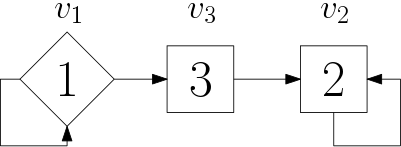
\includegraphics[scale=0.4]{counterexampleBconjecture}\\
\end{center}
All vertices are won by player $0$ ($v_1$ plays to $v_3$, $v_3$ must play to $v_2$ and $v_2$ must play to itself therefore we always get an infinite path of $v_2$'s).\\
We solve this game using \textsc{RecursivePG} and write down the values of relevant variables below. We use the hat decoration to indicate values for variables in the first recursion:\\
\begin{tabular}{|p{20cm}}
$\textsc{RecursivePG}(G)$:\\
$h=3$,$\alpha=1$\\
$A =\{v_3\}$\\
\begin{tabular}{|p{20cm}}
	$\textsc{RecursivePG}(G\backslash A)$:\\
	$\hat{h}=2,\hat{\alpha}=0$\\
	$\hat{A}=\{v_2\}$\\
	\begin{tabular}{|p{20cm}}
		$\textsc{RecursivePG}(G\backslash A\backslash \hat{A})$\\
	\end{tabular}
	$\hat{W}'_0 = \emptyset$\\
	$\hat{W}'_1 = \{v_1\} = \hat{W}'_{\overline{\hat{\alpha}}}$\\
	\textbf{Vertex $v_1$ is in $\hat{W}'_{\overline{\hat{\alpha}}}$ however in $G$ the vertex is won by player} $\hat{\alpha}$.\\
	$\hat{B} = \{v_1\}$\\
	\begin{tabular}{|p{20cm}}
		$\textsc{RecursivePG}(G\backslash A\backslash \hat{B})$\\
	\end{tabular}
	$\hat{W}''_0 = \{v_2\}, \hat{W}''_1 = \emptyset$\\
\end{tabular}
$W'_0 = W'_{\overline{\alpha}} = \{v_2\}$\\
$W'_1 = W'_\alpha = \{v_1\}$\\
$B = V$\\
$W_0 = V$
\end{tabular}

An algorithm that simply stops when $v_0$ is found to be won for player $\overline{\alpha}$ requires the above conjecture to be true, since this isn't the case such an algorithm is flawed. This problem is solved by using the $\Delta$ variable to get the \textsc{RecursivePGLocal} algorithm.
\subsection{Fixed-point iteration local}
The fixed-point iteration algorithm can be modified to locally solve a game for vertex $v_0$ by distinguishing two cases:
\begin{enumerate}
	\item If $d-1$ is even then the outermost fixed-point variable is a greatest fixed-point variable. When at some point $v_0 \notin Z_{d-1}$ then we know $v_0$ is never won by player $0$ and we are done.
	\item If $d-1$ is odd then the outermost fixed-point variable is a least fixed-point variable. When at some point $v_0 \in Z_{d-1}$ then we know $v_0$ is won by player $0$ and we are done.
\end{enumerate}